\documentclass[twocolumn,10pt]{article}

\usepackage[a4paper,hmargin=1.5cm,vmargin=2.5cm,]{geometry}
\setlength{\columnsep}{0.7cm}
\usepackage{palatino}
\usepackage{graphicx}
\usepackage[utf8]{inputenc}
\usepackage{hyperref}
\usepackage{minted}
\usemintedstyle{colorful}
\usepackage[font=small,labelfont=bf]{caption}
\urlstyle{same} % no tt font for URLs
\newcommand{\blockade}{\rule{3em}{0.7em}}  %% Marker for things to change before submission

\usepackage{natbib}
\bibliographystyle{genome_research}
\setcitestyle{aysep={}} 

\usepackage[dvipsnames]{xcolor}
\hypersetup{
    colorlinks,
    linkcolor={blue!50!black},
    citecolor={blue!50!black},
    urlcolor={blue!50!black}
}

\begin{document}

\setcounter{secnumdepth}{0}


\twocolumn[{%
\centering
\textbf{\Large R/LinkedCharts: A novel approach for simple but powerful interactive data analysis}
\vspace{1.5ex}

Svetlana Ovchinnikova and Simon Anders\\
{\footnotesize Center for Molecular Biology of the University of Heidelberg, Germany}
\vspace{1.5ex}

24 January 2020
\vspace{6ex}
}]

\section{Abstract}
In exploratory data analysis, one usually jumps back and forth between visualizations that provide overview of the whole data and others that dive into details. In data quality assessment, for example, it might be very helpful to have one chart showing a summary statistic for all samples, and clicking on one of the data points would display details on this sample in a second plot. Setting up such interactively linked charts is usually cumbersome and time-consuming to use them in ad hoc analysis. We present R/LinkedCharts, a framework  that renders this tasks radically simple: Producing linked charts is as quickly done as is producing conventional static plots in R, requiring a data scientist to write only very few lines of simple R code to obtain complex and general visualization. We expect that the convenience of our new tool will enable data scientists and bioinformaticians to perform much deeper and more thorough EDA with much less effort. Furthermore, R/LinkedCharts apps, typically first written as quick-and-dirty hacks, can also be polished to provide interactive data access in publication quality, thus contributing to open science.

\section{Introduction}

Problem of effective visualization has been there since the first reported experiment results. Continuously growing amount and complexity of available data over the last decades made it a challenging issue \citep{fisher_2017}. For a while the only available way to tackle the problem was to come up with more elaborate types of plots imploying colour, shape, transparensy and other visual aspects to combine multiple layers of information \citep{keahey_2013}. Yet, there are certain limits to how much information one can grasp from a static image. Excessive details and overcomplexity make visualization less interprateable. Thus a researcher is forced to make a decision on what information to keep when preparing figures for a paper or any other kind of report. From one hand, it is a good thing, since often data contains plenty of noise and information that is irrelevant to the point one tries to make. From the other hand, it may be complicated to make sure, that nothing of importance is missing in the graphical representation.

With the advance of mordern technologies, interactive visualisation emerged to offer a solution to this problem. In an interactive figure there is no need to make all aspects visible simultaneously or highlight everything of importance at once. Instead user is allowed to explore the figure in a quick and intuitive manner, concentrating at a time on the most interesting or suspicsious parts of the plot. Numerous tools now provide means of creating interactive visualizations not only for research, but for any area that involves data analisys and presentation of any sort \citep{caldarola_2017}. With their help one may avoid overburdening of figures without a need to put some information aside.

The advantage of interactivity lies beyond just simplifying navigation through big massives of data. When adding small changes to a plot takes just a click or two, it urges a researcher not to put aside ideas or concerns and thus go through the data more thoroughly. At the same time a possibility for readers to check conclusions and claims of a paper on the fly, without going through all the script and analysis, makes the paper more credible. Therefore, we believe that further integration of interactive tools in a researchers' routine can strongly improve quality of studies.

Today many papers offer an interactive resource as a way to present their data and results. Though these visualizations are often useful and provide a comprahensive insight into the data, they generally serve presentation purposes only. This means that only after completing main work on the project, researches spend a couple of days to deploy a nice interactive app to share their data and results with the scientific community. We, however, believe, that interactivity should also be used in every day tasks to facilitate data exploration. To this end, the tool to produce interactive apps should be both simple and highly customizeable.

Simplicity should serve as incentive to use interactivity whenever there is a smallest hint that it may be useful. If a tool is too complicated, one may prefer to do most of the analysis by more habitual static means, and wait for a special occasion when it's worthwhile to invest time into designing an interactive app. It should also be similar in design to most common visualization means, since tools with too specific interface tend to be used by people with more extensive programming skill. Even if a researcher with less expertise in coding has an eager-to-help colleague, he or she may be unwilling to ask for an assistance in minual every day tasks and wait for something big.

At the same time, an attempt to simplify a tool may result in hardcoding and presetting too many parameters. As a result, a simple-to-use tool can be applied to a single task it was designed for and any attempt of custamization, if at all possible, requires a considerable effort. Yet, it may be useful if one doesn't try to force a research problem in the predefined mould of a certain tool, but rather makes tool to fit a problem. This requires a reasonable degree of flexibility.

With the LinkedCharts, we've tried to find a ballance between the two goals of a tool for interactive data exploration. It requires only basic knowledge in R or JavaScript to produce fully functional apps that can be used for \emph{ad hoc} analysis. With a little more effort one can make a nicer looking app and customize most of commonly used plot settings (such as colours, labels, axes, etc.). And finally, with the time and skills that is generally required for the same task, one can use LinkedCharts to make a presentable app deployed on a server. Since the library is JavaScript based, it can be combined with various existing web solutions. One can also write cutom scripts that will change even hardcoded aspects of the library without making changes to the source code, thus making LinkedCharts extremely flexible. 

LinkedCharts is not fixed on any specific task. It is rather a toolbox and its blocks can be combined in any manner the same way as one combines plots for a complex paper figure. All block share the same interface and very similar interactivity capabilities, which means that understanding one of them is enough to grasp the entire concept of LinkedCharts.

With all these, we hope that LinkedCharts can become a useful asset for a scientific community that can be used both for everyday routine and for presenting one's reasearch to a greater audience. LinkedCharts available as an R package (\mintinline{R}{rlc}, can be downloaded from CRAN) and as a JavaScript library. This paper is focused on R implementation of LinkedCharts. 

\section{Results}
\subsection{Linking charts}

The main consept behind LinkedCharts is connecting to or more plots together so that manipulation with one of them affect the others. This process is what ``linked'' in ``LinkedCharts'' stands for. It can be better explained with a simple example based on data from \citet{conway_2015}.

\begin{figure*}
	\includegraphics[width=\textwidth]{FigD/figD.png}
	\caption{Overview of genes differentiall expressed in cancerous and normal tissues from \citet{conway_2015}. MA-plot (a) shows all the sequenced genes with their average expression on X-axis and log-fold change on Y-axis. Red indicates genes, where difference was reported as significant by ``limma'' package. Plot to the left (b) shows expression values (CPMs) for a selected gene (in this case LAMB4) and all the patients. This figure is based on a LinkedCharts app and it's live version can be found in a supplement. When user clicks on a point on the MA-plot, the expression plot changes, showing the new selected gene. This allows one to immediately check, whether the genes, labeled as significantly different, are in fact interesting for further study.}
	\label{FigD}
\end{figure*}

In this study, from each of 17 patients with oral cancer three samples were taken: one of normal tissue, one of tumour and one of displasia tissue. mRNA from all these samples was sequenced to obtain gene expression values. Now, one may ask what genes are significantly different between, let say, normal and cancerous tissues. Many packages offer functions to answer this question and for this example it is not important, which one to use. We've applied function \mintinline{R}{voom} from the ``limma'' \citep{ritchie_2015} package. To explore results of this function, it is common to make an MA-plot with the average gene expression on the x-axis and log fold change between the two groups on the y-axis (Fig \ref{FigD} (a)). Red dots correspond to genes that are considered significantly different between the two conditions (adjusted p.value < 0.1). The next natural question that may arise, is how the difference in expression looks like for every single patient. Is it persistent across all the patients or only detected in some of them? Are there any artifact or outliers that cause the p.value to be too small?

To find answers to these questions we can add another plot that shows expression values (CPM) for all the patients (Fig \ref{FigD}(b)). This plot can show expression for only one selected gene at a time, but LinkedCharts allows one to link it to the MA-plot. Now, any click on a point from the MA-plot makes the plot to the right to show expression of the corresponding gene. Fig \ref{FigD} is based on the LinkedCharts app, which can be found in the supplement of this paper. We encourage reader to pause for a moment and check it to get a feeling of LinkedCharts. There, we also provide full code to generate the app and links to necessary data files, so that one could immediately get this app in his or her R session and experiment with it. For this and all further examples we provide two versions of code: minimal with only essential parameters needed to make app functional, and more extended with custom colours, labels, etc. In the paper we will only focus on the minimal code.

To further explore the mechanism of linking, we can have a look at the code that generates the app from Fig \ref{FigD}. This is a minimal, but full code for the app. For now, we want to concentrate only on the highlighted lines.

\begin{minted}[highlightlines={2,9-12,17}]{R}
openPage(layout = "table1x2")
gene <- 1

lc_scatter(dat(
   x = AveExpr,
   y = tissuetumour,
   colour = ifelse(adj.P.Val < 0.1, 
                   "red", "black"),
   on_click = function(k) {
      gene <<- k
      updateCharts("A2")
   }),
"A1", with = voomResult)

lc_scatter(dat(
   x = patient,
   y = normCounts[gene, ],
   colourValue = tissue, 
   logScaleY = 10),
"A2", with = sampleTable)
\end{minted}

It works as follows. Somewhere in a variabe (\mintinline{R}{gene} in our case) we keep an index of the gene to show in the expression plot. This index is used to tell the chart, which line of the \mintinline{R}{normCounts} matrix (it is where normalized counts are stored) to use as y values of the plot: \mintinline{R}{y = normCounts[gene, ]}. Almost every chart of the R/LinkedCharts library has the \mintinline{R}{on_click} argument, which is a function, that will be called each time user clicks on an element of the plot (point, line, cell of a heatmap, etc.). In this example, whenever it happens, we change value of \mintinline{R}{gene} to index of the clicked point. Then we tell R/LinkedCharts to update the second plot (``A2'' is its ID set in the last line of the example). Updating means that all arguments inside the \mintinline{R}{dat()} function will be reevaluated and the chart will be changed accordingly. In our case, new value of \mintinline{R}{gene} will yield new y values for the expression plot.

This simple logic is not limited to just two plots and provide a base to create various apps both simple and complex. For example one of our tutorials (\url{https://anders-biostat.github.io/linked-charts/rlc/tutorials/citeseq1.html}) gives a detailed instructions to generate an app for sigle-cell data exploration. The app consists of four charts, three of which are scatter plots and one is an information table to show genes that define a selected cell cluster.

Besides reaction on a click, one may specify functions to be called when user moves mouse over or out of an element, selects or deselects elements with the Shift key pressed, clicks on any position of a plot or on a heatmap label (full list can be found on a man page for any function of the ``rlc'' package). Understanding of how to define these functions (above is shown a very typical example) is everything one needs to be abele to generate apps that run locally. Deeper knowledge is required only to deploy an R/LinkedCharts app on a server. 

\subsection{Basic syntax}

\begin{figure*}
	\includegraphics[width=\textwidth]{FigB/figB.png}
	\caption{Typical syntax of a R/LinkedCharts plot and its comparison with ggplot2 [ref] library as an example of one of the most commonly used plotting libraries. Lines of code are arranged so that same aspects of the charts are set next to each other. ``iris'' dataset, which is one the R built-in datasets, was used for this example. Both pieces of code are fully functional and their output is shown above the code.}
	\label{FigB}
\end{figure*}

Overall, we've tried to make R/LinkedCharts simple and recognizeable by any user even with a very basic knowledge of R. Any chart has a set of properties that each defines a single aspect of the chart. It can be already notices from the previous example, where vectors of values were used as x and y coordinates of points or their colours. The same principle is used in most plotting libraries. For example, Figure \ref{FigB} shows a comparison of syntax in R/LinkedCharts (``rlc'' package) and ggplot (``ggplot2'' package) for a simple scatter plot. Lines are arranged so that to match setting the same aspects of the plots, above the code there is its output. One can see, that structure of the input data is identical and there is hardly any difference between the two.

An important thing to notice here is the \mintinline{R}{dat()} function. Properties can be set in the same manner both inside and outside of it, but only those that are defined inside the \mintinline{R}{dat()} function will be evaluated on each call of \mintinline{R}{updateCharts} call. Everything outside this function will remain constant. There is a very small example that can illustrate the effect of the \mintinline{R}{dat()} function.

\begin{minted}{R}
lc_scatter(
   dat(x = rnorm(30)),
   y = rnorm(30))
\end{minted}

Running this code will produce a scatter plot with 30 randomly located points. Now, every time one calls \mintinline{R}{updateCharts()} x coordinates of each point will change to a new random value, but all the y coordinates will remain the same.

\begin{figure*}
	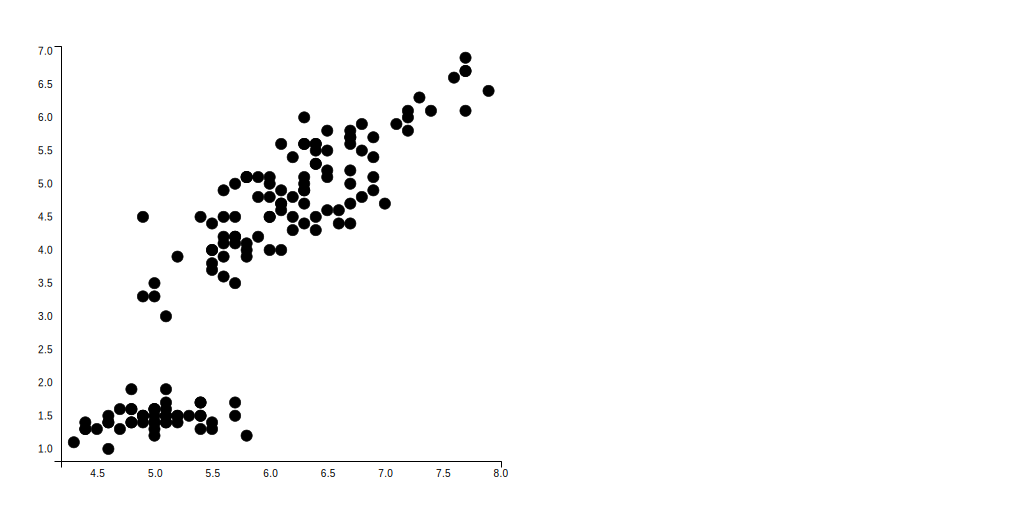
\includegraphics[width=\textwidth]{FigA/figA.png}
	\caption{Gallery of all available plotting functions the in \mintinline{R}{rlc} package. A scatter plot (a); a bee swarm plot (based on d3-beeswarm plugin [reference]) (b); a collection of various line plotting functions (c); a histogram and a density plot (density was multiplied by a factor of 500 to be visible on the same plot as the histogram) (d); a heatmap (e); a bar chart (f); a collection of interactive elements to gather input from user (g); functions to add custom HTML code and static plots to the page (h). All these examples with code to create them can be found in the supplement.}
	\label{FigA}
\end{figure*}

So far we've mentioned only scatter plots, but R/LinkedCharts is not limited by them alone. There are 15 main functions in the ``rlc'' package. Each of them generates a specific type of plot (such as scatter plot, heatmap, bar plot, etc.) or a navigation element (such as sliders or text fields). Figure \ref{FigA} shows them all together with some basic examples. Each plot, as it has been already mentioned, is defined by its properties: some of them are required (such as \mintinline{R}{x} and \mintinline{R}{y} for a scatter plot or \mintinline{R}{value} for a heatmap) many others are optional (\mintinline{R}{palette}, \mintinline{R}{title}, \mintinline{R}{ticks} etc.). A full list of all the properties with live examples is available at \url{https://anders-biostat.github.io/linked-charts/rlc/tutorials/props.html} and also on the R man page for each plotting function. Many of the properties accept minor variations in spelling (\mintinline{R}{colour/color} or \mintinline{R}{labels/label}).

\subsection{Use Cases}
\subsubsection{Quality check}

It is common that on the way from obtaining raw data towards meaningful conclusions one undertakes a number of steps, each involving some data condensing and inevitable information loss. For example, raw reads in RNA-seq are aligned and counted to produce gene expression values for each sample or cell. However, quality of reads and confidence of alignment is no longer included in the data. The next step can be, for example, to find nearest neighbours or to calculate a distance matrix to be further used for clustering or visualization. This makes data even more interpreteable, but now we no longer use information on individual expression levels. 

Of course, information that is put aside is not only used to produce the next step values, but also to perform various quality checks. Low-quality reads are usually removed from the study as well as samples that show abnormal expression patterns. We tend to believe that we no longer care about those pieces of data that are left behind in the research flow, since we've already taken everything we need from them. Yet, especially in studies involving big data, these checks are automated. The researcher only looks at some summarized reports and may also have a look at some random examples. If those look reasonable, the general assumption is that all the data that was not filtered out is also reasonable. However, while there is only one way for everything to be right, there are numerous ways for the data to be either wrong or just not like one has expected. Therefore, it's important to be able to look back, before making any kind of conclusions from a figure that show a condenced result.

This idea is the main motivation behind the LinkedCharts library. It is illustrated in the Figure \ref{FigC}. If we have a workflow or a pipeline, that performs certain transformations of the data, LinkedCharts offers an easy way to look back through each of the steps. Whenever a researcher encounters an interesting or suspicious pattern in the data, he or she can with minimal effort check  whether it is a real biological finding or some technical artifact, missed by quality checks. 

\begin{figure*}
	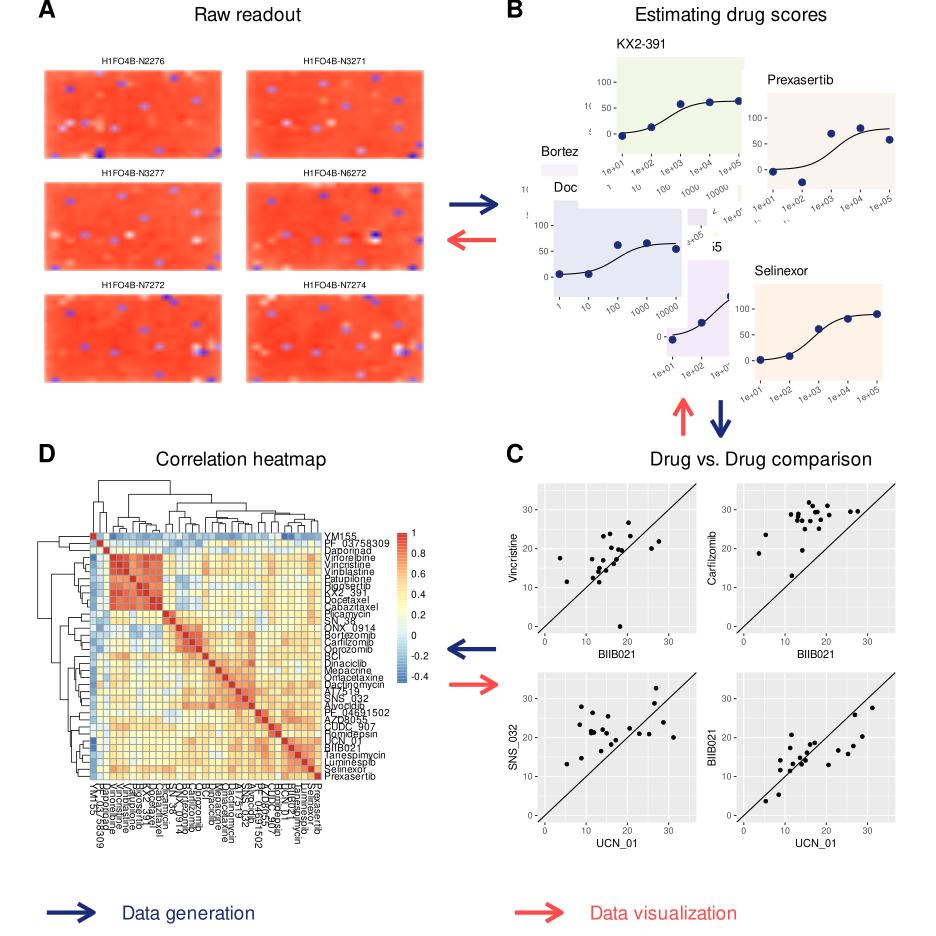
\includegraphics[width=\textwidth]{FigC/figC.png}
	\caption{Main idea behind the LinkedCharts library is shown based on a drug screening experiment. Blue arrow shows a direction of a common pipeline. We start with reading intensity values from plates with different cell lines, grown in the presence of a number drugs in different concentrations (A). These values are then normalized and aggregated to yield a single score for each drug (B). The scores of different drugs are compared to each other across all the tested cell lines (C). A drug-drug correlation heatmap is then produced to identify clusters of similar drugs (D). This pipeline is a simplified version of study from [reference? Have they published that by now?] for demonstration purposes. The live app and related code can be found in the supplement.}
	\label{FigC}
\end{figure*}

R/LinkedCharts is particularly effective in generating a chain of ``linked'' charts, where a chart explains each element of the previous one. For example, in our first app from the ``Linking cahrts'' section, one of the scatter plots explains each point of the other one. When a point on the MA-plot is clicked, we can see expression of the corresponding gene for all the patients. Therefore, it "explains", why we see or don't see a significant difference in expression for the given gene. We can continue the chain of charts and, for instance, add some information about each patient such as clinical data if available. 

Another example is shown in Figure \ref{FigC} and also is available in the supplement. It is based on the data from [reference].
For demonstration purposes, we use only a subset of available data here to simulate a typical drug-screening pipeline. In this subset 50 drugs each in five different concentrations were tested against 17 pancreatic cancer cell lines. The main heatmap shows drug-drug correlation values. By clicking on a cell of the heatmap user selects two drugs and can check individual drug scores (?) of each of them against all the tested cell lines. The inhibition values were calculated based on drug activity in five tested concentrations. So the third plot shows all those activity levels for each conentration. Finally, one can also find raw readouts from the plates in order to check for plate-related effects if any. In this manner each chart represents one of the major steps of the pipeline taht led from plate readouts to a correlation hetmap that highlights clusters of drugs with similar behavioural patterns. More details as well as code and links to download the data one can find in the supplement. 

Such apps would allow a quick and easy spot check of uncovered data patterns and can give researcher a better way to understand inner connections between the data. For instance, to what extent noise can influence the signal or what scale of changes in the value of interest is typical to the data.

\subsubsection{Exploratory analysis}

While interactivity is already heavily used for presenting study results to the research community, with R/LinkedCharts we would like to emphasize its advantages for everyday exploratory analysis. To this end we've made an effort to make it possible for a user to get interactive apps with not more effort than is usually required to get a static plot.

\begin{figure*}
  \includegraphics[width=\textwidth]{FigE/figE.png}
  \caption{Examples of simple plots that are commonly used during exploratory analisys with the code to produce them. Basic plots of ``rlc'' (c, d) package are not more complicated than their static alternatives (a, b), which makes R/LinkedCharts suitable for every day on-the-fly analisys. For static heatmap (a), the ``pheatmap'' package was used; scatter plot (b) was made with a base R function. The heatmaps (a, c) show Spearman correlation of gene expression for all samples from \citet{conway_2015}. To the right from the heatmaps there is gene expression from the two samples (normal and dysplasia tissues from the same patient) plotted against each other (b, d). Normal tissue sample (along x-axis) is one of the outliers that can be seen on any of the heatmaps (the samples that have lower then average correlation in the dataset with all other samples). Here, we consider such simple scatter plots as the quickest way of trying to see what is different about some of the samples. For the sake of simplicity, gene expression for all the samples is subsetted to 8000 randomly selected genes.}
  \label{FigE}
\end{figure*}
 
For example, let's again have a look at the oral cancer data \citep{conway_2015}. There are overall 57 samples, three from each patient. Previously, we've looked at differentially expressed genes between normal and cancerous tissues, but before getting there a researcher who's just got these data may want to get some overview of the samples. One of the common ways to do so is to check how well the samples are correlated with each other by making a correlation heatmap. Assume that we store sample correlation matrix in a, let say, \mintinline{R}{corMat} variable. In Figure \ref{FigE} are shown a static heatmap from a popular ``pheatmap'' package (a) and an interactive heatmap from ``rlc'' (c). Above each heatmap there is a command that generates it. Both commands look similarly simple and the only big difference in the output is that the rows and columns of the static heatmap (a) are clustered. However, hierarchical clustering is also implemented in R/LinkedCharts heatmaps, but is off by default unlike in pheatmap. One can control it with the same arguments \mintinline{R}{clusterRows} and \mintinline{R}{clusterCols} as in ``pheatmap''.

From any of the heatmaps we can see, that some of the samples are very much different from all others. The next thing one can ask is what is wrong with them. For the first and quick \emph{ad hoc} check one may decide to plot gene expression in several samples against each other to see if any noticeable patterns will hint a direction for further analysis. Let's say, that by looking at the heatmap, we've decided to start with plotting samples ``PG123-N'' and ``PG123-D''. These are normal and dysplasia samples from the same patients respectively and the normal one is one of the noticeable outliers.

\begin{minted}{R}
xSample <- "PG123-N"
ySample <- "PG123-D"
\end{minted}

Simple scatter plots from base R and ``rlc'' to compare normalized gene expression for both of the samples are shown in Figure \ref{FigE} (b, d) together with the code to produce them. Once again, both code lines are simple enough to be used for some quick on-the-fly checks.

This comparison alone doesn't tell us much, unless we look plot more samples against each other to see how expression for other samples look like, what is "high correlation" for this dataset and what is "low correlation". To this end we will have to store some other sample IDs to \mintinline{R}{xSample} and \mintinline{R}{ySample} variables and rerun the code to generate scatter plots again. Here comes the first point, where interactivity can facilitate exploration. If you surround \mintinline{R}{x} and \mintinline{R}{y} arguments of \mintinline{R}{lc_scatter} with the \mintinline{R}{dat} function, you can update the scatter with a call to the \mintinline{R}{updateCharts} function instead of rerunning the code. The full code will look like this:

\begin{minted}{R}
xSample <- "PG123-N"
ySample <- "PG123-D"

lc_scatter(dat(x = normCounts[, xSample], 
   y = normCounts[, ySample]),
   size = 1.5)

xSample <- "PG123-T"
updateCharts()
\end{minted}

If one is going to check multiple pairs of samples, it's only natural to put the last two lines in a function, that takes two samples and plots them agains each other.

\begin{minted}{R}
changePlots <- function(x, y) {
  xSample <- x
  ySample <- y
  updateCharts()
}
\end{minted}

At this point, we still need to decide what samples to plot and manually type in their names or indices. This can be avoided simply by supplying this function to the heatmap. Now, instead of entering sample names one can just click on a heatmap cell and it's row and column indices will be automatically given to the function and the scatter plot will be updated. As a result, we've made a functional interactive app with only the step that one may anyway perform during a routine exploratory analisys. The resulting code is shown below. You can also find a little bit prettified live version in the supplement and use it to see that the outlier samples are the ones that were sequenced less deep.

\begin{minted}{R}
lc_heatmap(value = corMat,
   on_click = function(d) {
      xSample <<- d[1]
      ySample <<- d[2]
      updateCharts()
   })
lc_scatter(dat(x = normCounts[, xSample], 
   y = normCounts[, ySample]),
   size = 1.5)
\end{minted}

\subsubsection{Server apps}

Any R/LinkedCharts app starts a server that listens to a given or randomly chosen port. A request from any browser for a starting page to this server will be answered with all the charts user has added so far. In practice it means that any R/LinkedCharts app can be accessed by multiple users, if they can make request to the server, and this doesn't require any additional parameters to be set. Any of the examples, we've shown in different sections of this paper can become apps that are deployed on a server.

For the complete functionality, there is just one thing that is needed to taken care of. If you once again take a look at the code for previously mentioned examples, you can notice that there is usually one or several ``state'' variables. These are gerenally global variables that store currently selected genes, samples, etc. and are changed inside callback functions: \mintinline{R}{gene} from the example in section "Linking charts", \mintinline{R}{xSample} and \mintinline{R}{ySample} from the example in the previous section. Now, if several users are accessing these apps simultaneously, each click will change the state variables and therefore changing charts for all the users. This still may be usefull if, for example, several people are using the app as a visual addition to an online meeting. Yet in most cases one would like interactivity to be independent for each user.

To this end, one need just to specify the state variables within the \mintinline{R}{openPage} function and give them some default values. For instance, example from the previous section can be turned into a server app simply by adding the following line in the beginning.

\begin{minted}{R}
openPage(sessionVars = list(xSample = 1, ySample = 2))
\end{minted}

Now, multiple users can work with an individual state of the app.

Of course, there are other things that can make a server app more customized. One can add some default content to each opened page (in addition to all the charts that are added by default), control each client session (and, for example, close those, that don't show any activity for considerable amount of time), limit memory usage or number of active connections simultaneously. Yet, all these parameters are optional. More information about possible options can be found on R man pages for classes \mintinline{R}{App} and \mintinline{R}{Session} of our ``jrc'' package.

\subsubsection{Stand-alone apps}

\begin{figure*}
  \includegraphics[width=\textwidth]{FigF/figF.png}
  \caption{An example of a stand-alone app with LinkedCharts. The app was used as a supplement for (reference)}
  \label{FigF}
\end{figure*}

Any app made with R/LinkedCharts (``rlc'' package) requires an R session that runs either locally or on the server. Yet, R session is only responsible for sending required data to the app, while all the visualization and interactivity handling happens on the JavaScript side. This fact makes it possible to use LinkedCharts for generating stand-alone apps in a form of an HTML page. Such a page can then be sent to a collaborator or used as a supplement file for a paper. Unlike a link to an app deployed somewhere on a server, this kind of interactive supplement will be awaylable to any user with an installed web-browser at any moment, without a need for the research team to maintain a runnig app on the server. A supplement to this paper is an example of such an app, contained within an HTML page. Another app was made for (referece to translation paper). A screenshot of this app is shown in Figure \ref{FigF}.

However, to make such an app one has to be familiar with JavaScript. We've tried to make the necessary level of experience with JavaScript as low as possible, but understanding of syntax and some basic concepts is still required. In the supplement to this paper you can also find JS code for all the apps. The data has to be preprocessed (alternatively, all the calculations may be implemented in JavaScript, but that can be complicated) and saved, for example, in JSON format. The result can be directly inserted into the JS code. There are also ohter ways of loading data into the linked-charts.js app, which are described in our tutorial https://anders-biostat.github.io/linked-charts/js/tutorials/data.html. Also on this web-page one can find more tutorials and examples for a JavaScript part of the LinkedCharts library.

\subsection{Further customization}

Since LinkedCharts is JavaScript based, it can be combined with many existing web solutions without changing source code of the package. One can cultomize how the charts look like with CSS, add additional scripts, specify an HTML layout. R/LinkedCharts can add interactive charts to an existing HTML page supplied as \mintinline{R}{startPage} argument of the \mintinline{R}{openPage}. Additional images, files or scripts can be loaded from a directory specified by the \mintinline{R}{rootDirectory} argument. And finally, the ``jrc'' package (available on CRAN) on top of which ``rlc'' is built allows you to run any JavaScript code directly from your R session.
All this gives you full control of how your app looks like and behaves and can be fitted to the specific needs of your current project.

\begin{small} 
\balance
\bibliography{lc}
\end{small}

\end{document}


